\section{Discount usability evaluation method}
When we refer to the discount evaluation method, we mean the cooperative evaluation created by Andrew Monk et al., 1993\cite{AndrewMonk}. \tabref{fig:UsabilityTable} from Designing Interactive Systems\cite{CooperativeEval} outlines the steps from the method.

\begin{figure}[]
  \centering      
    \begin{subfigure}[b]{\textwidth}
    \begin{center}
      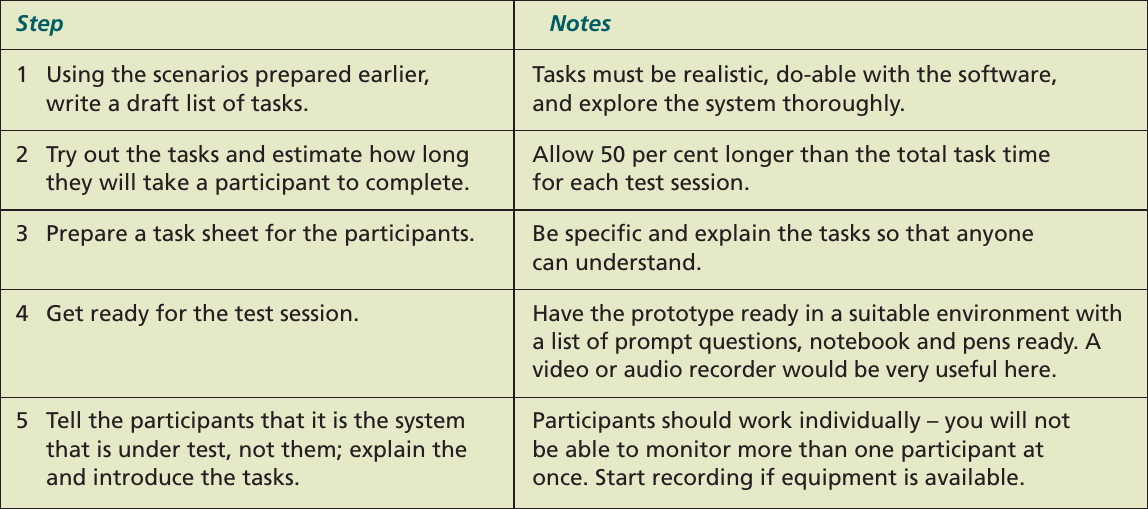
\includegraphics[scale=0.5]{./pics/UsabilityTableP1}
      \caption{table part 1}
      \label{fig:UsabilityTableP1}
    \end{center}
    \end{subfigure}
    ~\\
    \begin{subfigure}[b]{\textwidth}
    \begin{center}
      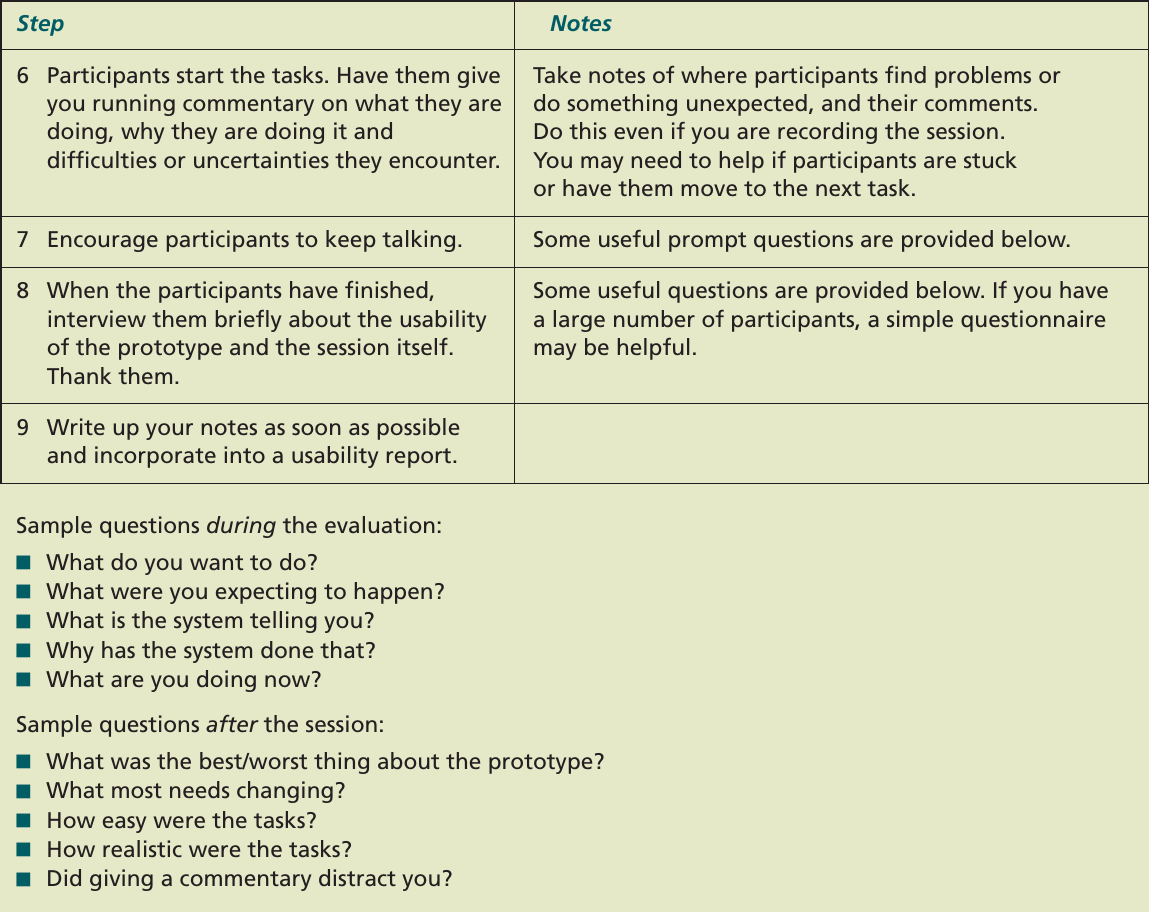
\includegraphics[scale=0.5]{./pics/UsabilityTableP2}
      \caption{table part 2}
      \label{fig:UsabilityTableP2}
    \end{center}
    \end{subfigure}
    \caption{combined caption}
    \label{fig:UsabilityTable}
\end{figure}

The method is focused on finding the more impactful usability problems over finding a lot of them, and has thus proven to be both lightweight and useful. In particular, the Nielsen Norman Group\cite{5Users} shows that you only need about 5 test subjects to get clear feedback on your system. Jakob Nielsen argues that instead of expending huge budget and time, the best results could be achieved by conducting multiple smaller tests. In their experiments across a large number of projects, one test subject managed to find roughly 31\% of the the existing usability problems. Every subsequent user contributes to the curve by identifying new problems, but that also includes problems already found by the previous user. Technically, after a certain point, adding additional users contribute less and less to the overall identification of problems, having essentially diminishing returns. The curve presented by the author shows that 15 test users are needed to identify all the usability problems. However, since the goal usually is to improve the design rather than document its weaknesses, they recommend conducting 3 smaller tests with 5 users each rather than one experiment with all 15 users.